\section{Eksperyment}
    \subsection{Założenia}
    Podczas przeprowadzania eksperymentu należało pamiętać o następujących założeniach:
    \begin{itemize}
        \item{sprawdzenie 3 zbiorów danych: \textbf{Diabetes}, \textbf{Glass} oraz \textbf{Wine},}
        \item{zbadanie 3 metod dyskretyzacji (tutaj: \textbf{equal-width}, \textbf{equal-frequency}
              oraz \textbf{CAIM}) lub założenie, że dane mają \textbf{rozkład normalny},}
        \item{zbadanie wpływu \textbf{paramteru kroswalidacji} dla zwykłej oraz \textbf{stratyfikowanej},}
        \item{zbadanie i wyciągnięcie wniosków z dostępnych miar oceny jakości klasyfikatora
              (\textbf{accuracy}, \textbf{precision}, \textbf{recall}, \textbf{f1} oraz \textbf{confusion matrix}}
    \end{itemize}
    Szczegółowe wyniki (wykresy, tabelki) tego eksperymentu są przedstawione w kolejnych podrozdziałach.

    \subsection{Wyniki dyskretyzacji}


\subsubsection{Zbiór danych - "Diabetes"}
    \begin{figure}[H]
        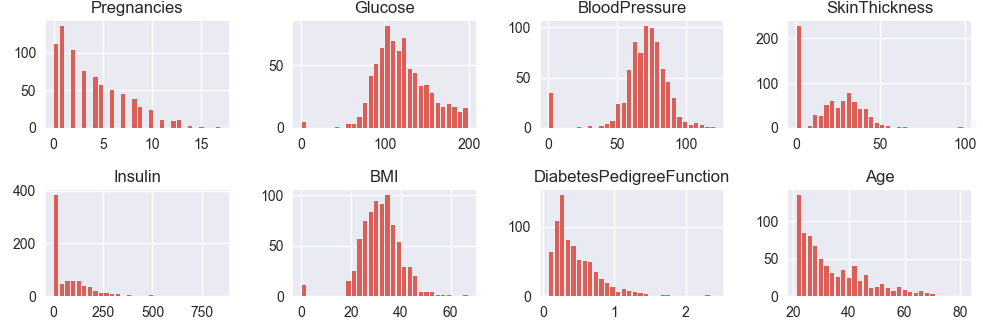
\includegraphics[width=\textwidth]{img/discretization/non_discretized_diabetes.png}
        \caption{Rozkłady atrybutów zbioru "Diabetes" -- brak dyskretyzacji.}
    \end{figure}

    \begin{figure}[H]
        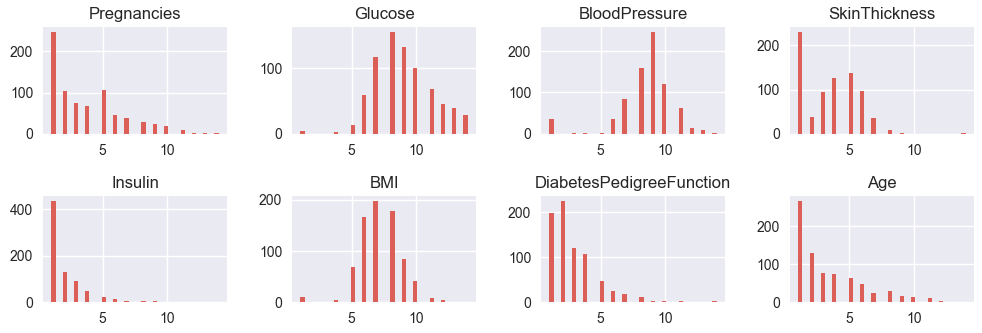
\includegraphics[width=\textwidth]{img/discretization/ew_diabetes.png}
        \caption{Rozkłady atrybutów zbioru "Diabetes" -- dyskretyzacja "equal-width".}
    \end{figure}

    \begin{figure}[H]
        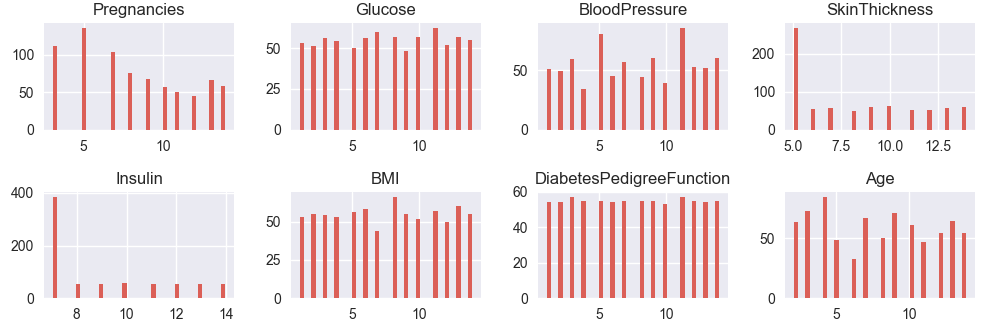
\includegraphics[width=\textwidth]{img/discretization/ef_diabetes.png}
        \caption{Rozkłady atrybutów zbioru "Diabetes" -- dyskretyzacja "equal-frequency".}
    \end{figure}

    \begin{figure}[H]
        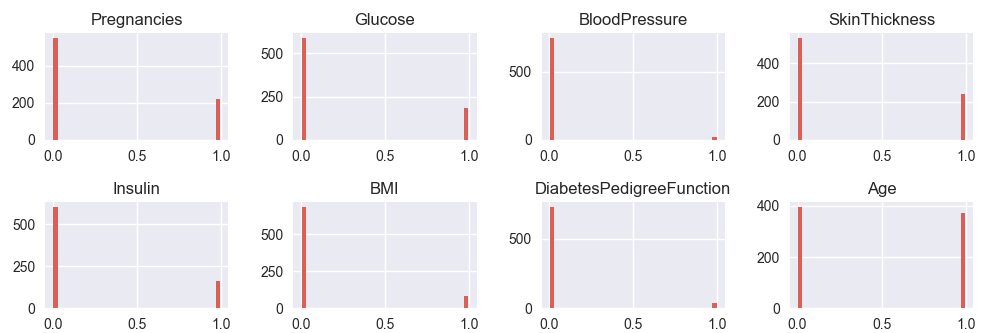
\includegraphics[width=\textwidth]{img/discretization/caim_diabetes.png}
        \caption{Rozkłady atrybutów zbioru "Diabetes" -- dyskretyzacja "CAIM".}
    \end{figure}

\subsubsection{Zbiór danych - "Glass"}
    \begin{figure}[H]
        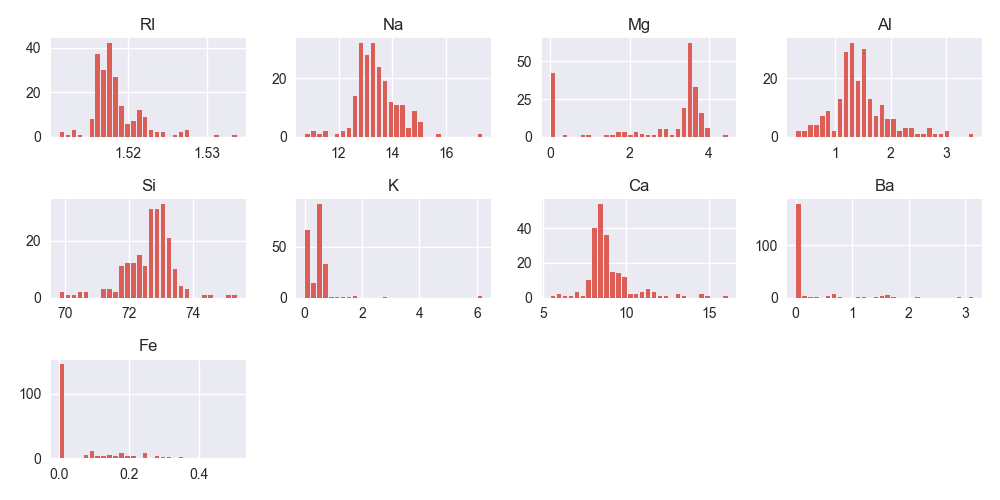
\includegraphics[width=\textwidth]{img/discretization/non_discretized_glass.png}
        \caption{Rozkłady atrybutów zbioru "Glass" -- brak dyskretyzacji.}
    \end{figure}

    \begin{figure}[H]
        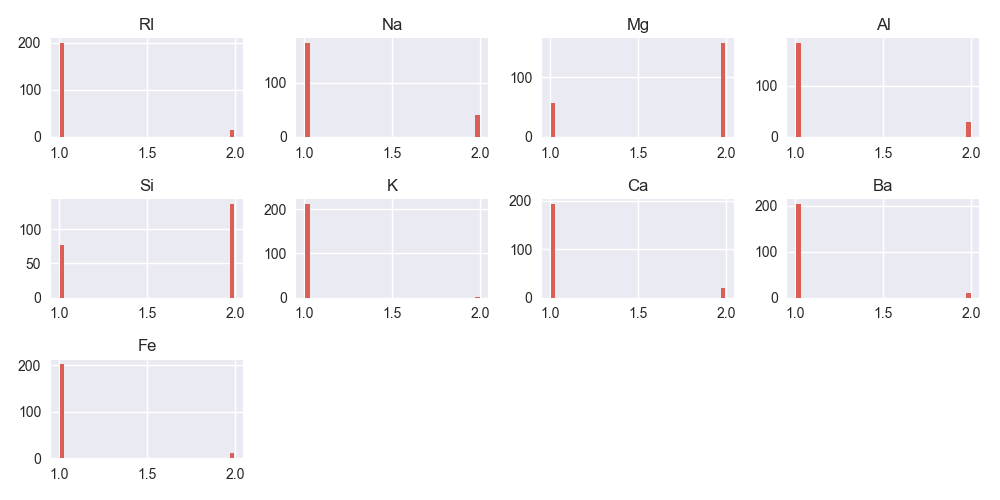
\includegraphics[width=\textwidth]{img/discretization/ew_glass.png}
        \caption{Rozkłady atrybutów zbioru "Glass" -- dyskretyzacja "equal-width".}
    \end{figure}

    \begin{figure}[H]
        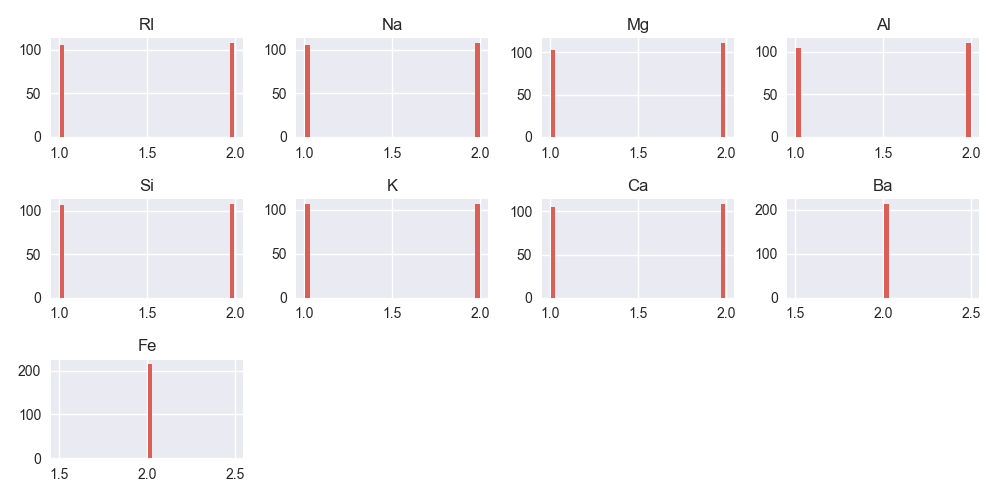
\includegraphics[width=\textwidth]{img/discretization/ef_glass.png}
        \caption{Rozkłady atrybutów zbioru "Glass" -- dyskretyzacja "equal-frequency".}
    \end{figure}

    \begin{figure}[H]
        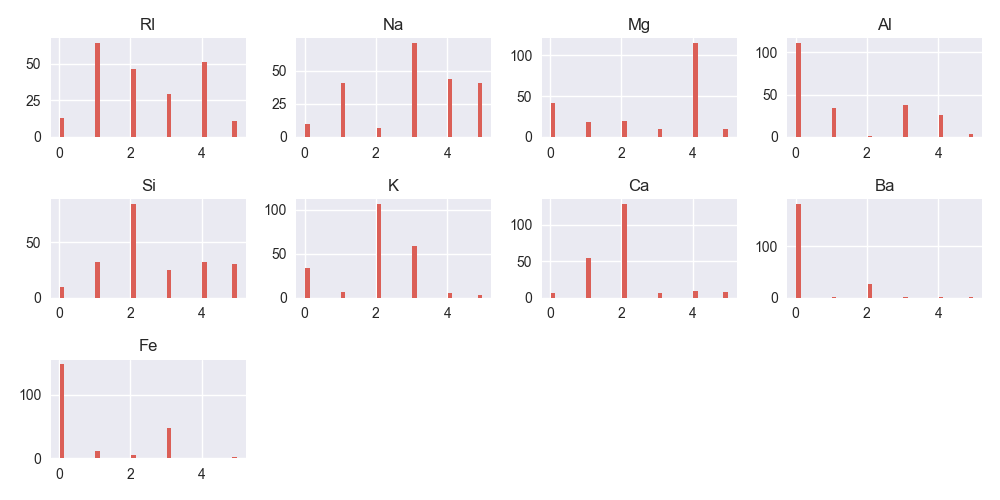
\includegraphics[width=\textwidth]{img/discretization/caim_glass.png}
        \caption{Rozkłady atrybutów zbioru "Glass" -- dyskretyzacja "CAIM".}
    \end{figure}
    
    
\subsubsection{Zbiór danych - "Wine"}
    \begin{figure}[H]
        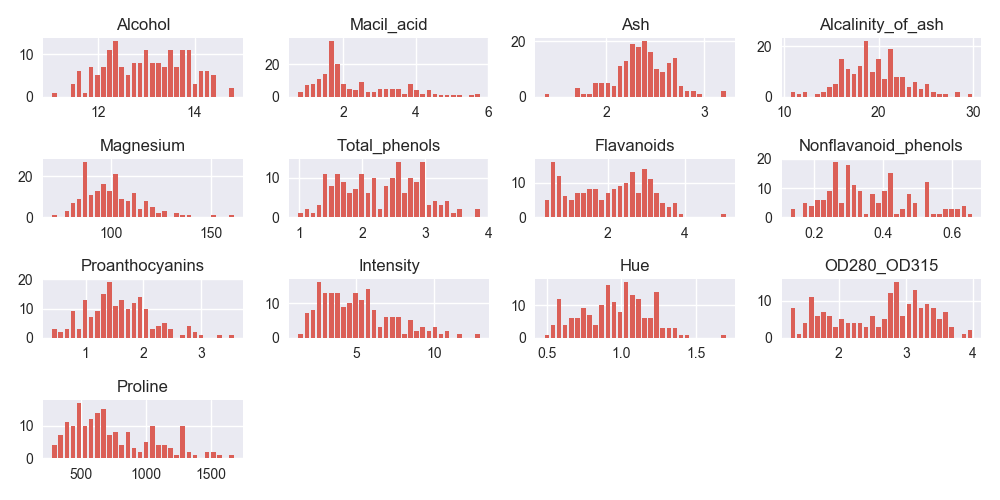
\includegraphics[width=\textwidth]{img/discretization/non_discretized_wine.png}
        \caption{Rozkłady atrybutów zbioru "Wine" -- brak dyskretyzacji.}
    \end{figure}

    \begin{figure}[H]
        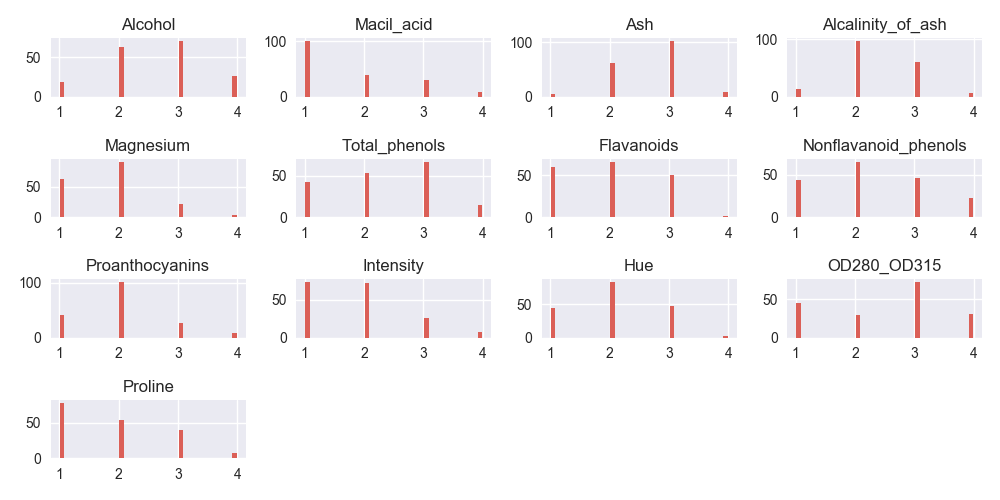
\includegraphics[width=\textwidth]{img/discretization/ew_wine.png}
        \caption{Rozkłady atrybutów zbioru "Wine" -- dyskretyzacja "equal-width".}
    \end{figure}

    \begin{figure}[H]
        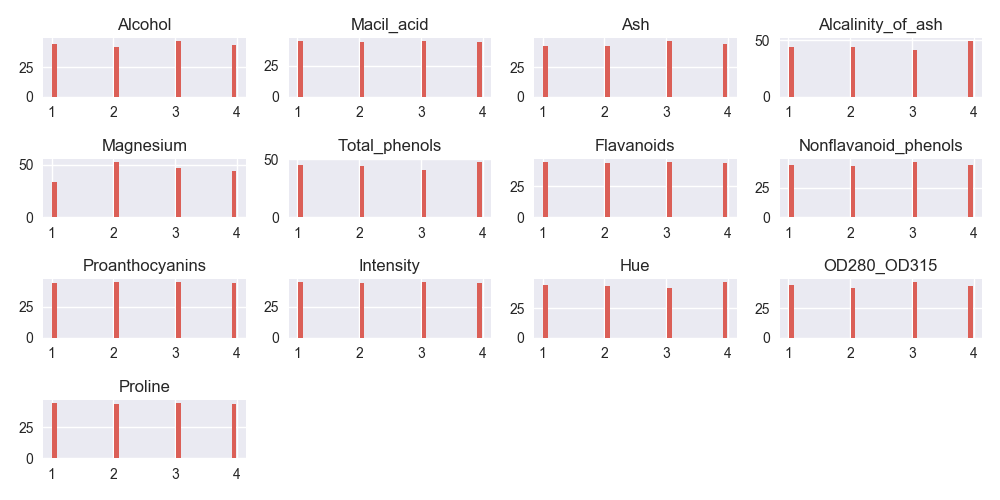
\includegraphics[width=\textwidth]{img/discretization/ef_wine.png}
        \caption{Rozkłady atrybutów zbioru "Wine" -- dyskretyzacja "equal-frequency".}
    \end{figure}

    \begin{figure}[H]
        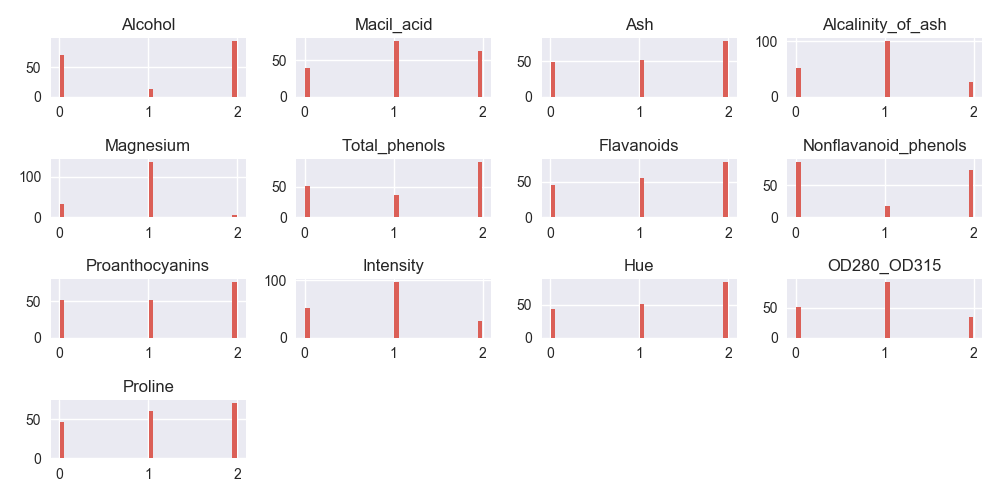
\includegraphics[width=\textwidth]{img/discretization/caim_wine.png}
        \caption{Rozkłady atrybutów zbioru "Wine" -- dyskretyzacja "CAIM".}
    \end{figure}

    \pagebreak
\subsection{Wyniki kroswalidacji}
    Poniżej zostały przedstawione wyniki zastosowania kroswalidacji (z parametrem
    w postaci liczby podzbiorów; zmieniający się od 2 do 9 ze skokiem 1) zbiorów danych,
    które:
    \begin{itemize}
      \item{}
    \end{itemize}
    a następnie w ramach danego procesu kroswalidacji, wyznaczono wartości miar
    oceny jakości klasyfikatora. Dodatkowo zostały zamieszczone tabelki z dokładnymi
    wartościami tych miar.

    \subsubsection{Zbiór danych -- "Diabetes"}
        \begin{figure}[H]
    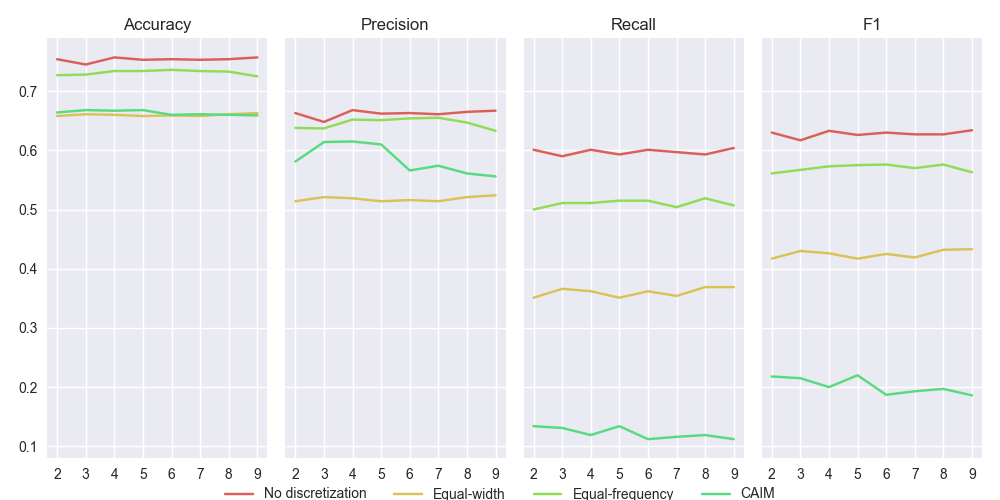
\includegraphics[width=\textwidth]{img/cv_scores_kfold/scoring_kfold_diabetes.png}
    \caption{Wykresy wartości metryk dla zbioru "Diabetes" -- krowalidacja zwykła.}
\end{figure}

 \begin{table}[H]
    \center
    \caption{Wartości metryk dla zbioru "Diabetes" -- krowalidacja zwykła.}
    \begin{tabular}{|c|c|c|c|c|c|c|c|c|c|}
        \hline
        \multirow{2}{*}{\textbf{Metoda dyskr.}} & \multirow{2}{*}{\textbf{Metryka}} & \multicolumn{8}{|c|}{\textbf{CV}} \\ \cline{3-10}
                                                &  & 2 & 3 & 4 & 5 & 6 & 7 & 8 & 9 \\ \hline
            \multirow{4}{*}{\textit{Brak}}  & Accuracy & 0.754 & 0.745 & 0.757 & 0.753 & 0.754 & 0.753 & 0.754 & 0.757 \\ \cline{2-10}
                                             & Precision & 0.663 & 0.648 & 0.668 & 0.662 & 0.663 & 0.661 & 0.665 & 0.667 \\ \cline{2-10}
                                             & Recall & 0.601 & 0.59 & 0.601 & 0.593 & 0.601 & 0.597 & 0.593 & 0.604 \\ \cline{2-10}
                                             & F1 & 0.63 & 0.617 & 0.633 & 0.626 & 0.63 & 0.627 & 0.627 & 0.634 \\ \hline  \hline


                                            \multirow{4}{*}{\textit{Equal-width}}  & Accuracy & 0.658 & 0.661 & 0.66 & 0.658 & 0.659 & 0.658 & 0.661 & 0.663 \\ \cline{2-10}
                                             & Precision & 0.514 & 0.521 & 0.519 & 0.514 & 0.516 & 0.514 & 0.521 & 0.524 \\ \cline{2-10}
                                             & Recall & 0.351 & 0.366 & 0.362 & 0.351 & 0.362 & 0.354 & 0.369 & 0.369 \\ \cline{2-10}
                                             & F1 & 0.417 & 0.43 & 0.426 & 0.417 & 0.425 & 0.419 & 0.432 & 0.433 \\ \hline  \hline


                                            \multirow{4}{*}{\textit{Equal-freq}}  & Accuracy & 0.727 & 0.728 & 0.734 & 0.734 & 0.736 & 0.734 & 0.733 & 0.725 \\ \cline{2-10}
                                             & Precision & 0.638 & 0.637 & 0.652 & 0.651 & 0.654 & 0.655 & 0.647 & 0.633 \\ \cline{2-10}
                                             & Recall & 0.5 & 0.511 & 0.511 & 0.515 & 0.515 & 0.504 & 0.519 & 0.507 \\ \cline{2-10}
                                             & F1 & 0.561 & 0.567 & 0.573 & 0.575 & 0.576 & 0.57 & 0.576 & 0.563 \\ \hline  \hline


                                            \multirow{4}{*}{\textit{CAIM}}  & Accuracy & 0.664 & 0.668 & 0.667 & 0.668 & 0.66 & 0.661 & 0.66 & 0.659 \\ \cline{2-10}
                                             & Precision & 0.581 & 0.614 & 0.615 & 0.61 & 0.566 & 0.574 & 0.561 & 0.556 \\ \cline{2-10}
                                             & Recall & 0.134 & 0.131 & 0.119 & 0.134 & 0.112 & 0.116 & 0.119 & 0.112 \\ \cline{2-10}
                                             & F1 & 0.218 & 0.215 & 0.2 & 0.22 & 0.187 & 0.193 & 0.197 & 0.186 \\ \hline  \hline
            \hline
        \end{tabular}
    \end{table}

\begin{figure}[H]
    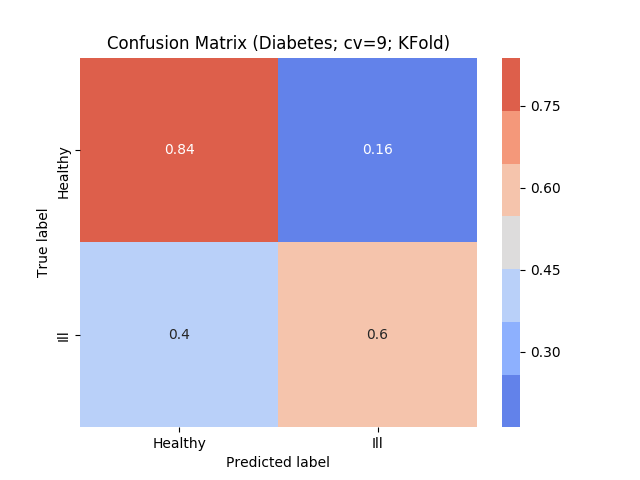
\includegraphics[width=\textwidth]{img/conf_matrices/cm_Diabetes_cv9_KFold.png}
    \caption{Macierz konfuzji dla najlepszej wartości F1 -- kroswalidacja zwykła.}
\end{figure}
        \begin{figure}[H]
\center
    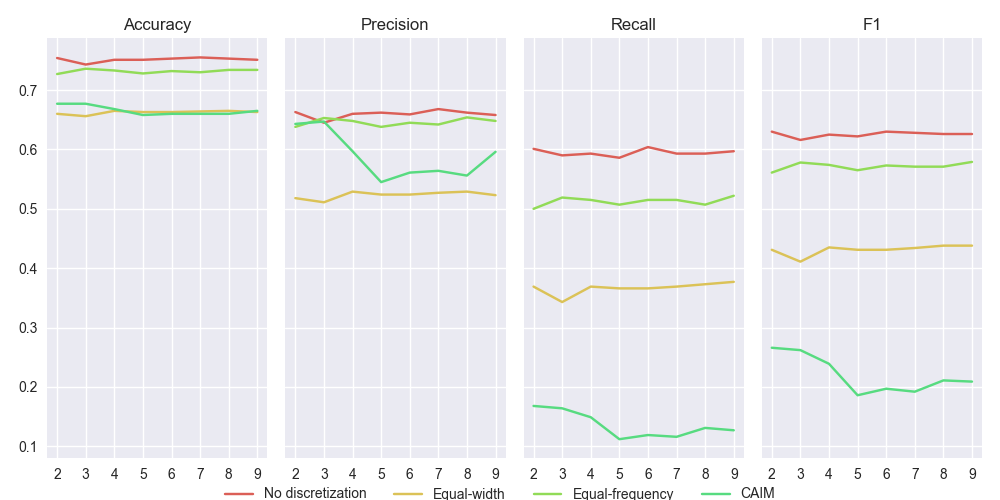
\includegraphics[width=\textwidth]{img/cv_scores_stratifiedkfold/scoring_stratifiedkfold_diabetes.png}
    \caption{Wykresy wartości metryk dla zbioru "Diabetes" -- kroswalidacja stratyfikowana.}
\end{figure}



    \pagebreak
    \subsubsection{Zbiór danych -- "Glass"}
        \begin{figure}[H]
    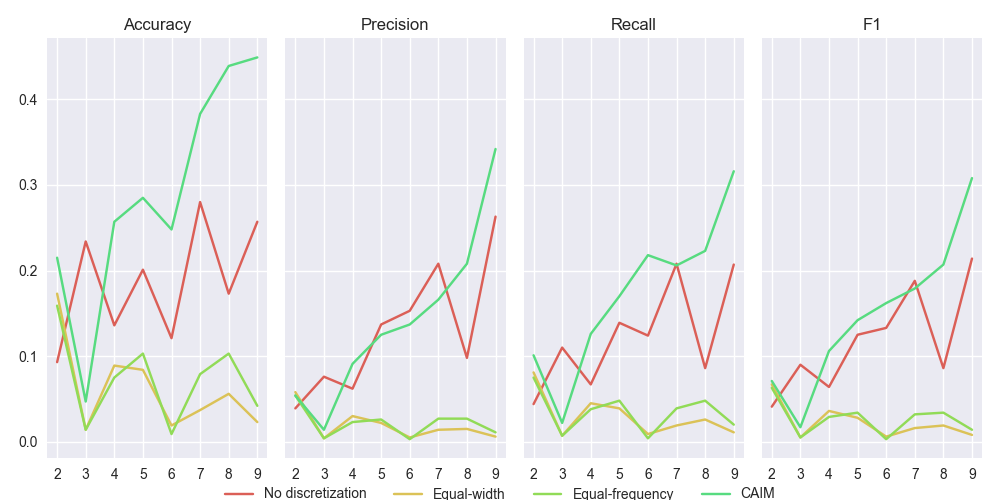
\includegraphics[width=\textwidth]{img/cv_scores_kfold/scoring_kfold_glass.png}
    \caption{Wykresy wartości metryk dla zbioru "Glass" -- krowalidacja zwykła.}
\end{figure}

\begin{table}[H]
\center
\caption{Wartości metryk dla zbioru "Glass" -- krowalidacja zwykła.}
    \begin{tabular}{|c|c|c|c|c|c|c|c|c|c|}
        \hline
        \multirow{2}{*}{\textbf{Metoda dyskr.}} & \multirow{2}{*}{\textbf{Metryka}} & \multicolumn{8}{|c|}{\textbf{CV}} \\ \cline{3-10}
                        &  & 2 & 3 & 4 & 5 & 6 & 7 & 8 & 9 \\ \hline
        \multirow{4}{*}{\textit{Brak}}  & Accuracy & 0.093 & 0.234 & 0.136 & 0.201 & 0.121 & 0.28 & 0.173 & 0.257 \\ \cline{2-10}
                                         & Precision & 0.039 & 0.076 & 0.062 & 0.137 & 0.153 & 0.208 & 0.098 & 0.263 \\ \cline{2-10}
                                         & Recall & 0.044 & 0.11 & 0.067 & 0.139 & 0.124 & 0.208 & 0.086 & 0.207 \\ \cline{2-10}
                                         & F1 & 0.041 & 0.09 & 0.064 & 0.125 & 0.133 & 0.188 & 0.086 & 0.214 \\ \hline \hline


        \multirow{4}{*}{\textit{Equal-width}}  & Accuracy & 0.173 & 0.014 & 0.089 & 0.084 & 0.019 & 0.037 & 0.056 & 0.023 \\ \cline{2-10}
                                                 & Precision & 0.058 & 0.004 & 0.03 & 0.022 & 0.005 & 0.014 & 0.015 & 0.006 \\ \cline{2-10}
                                                 & Recall & 0.081 & 0.007 & 0.045 & 0.039 & 0.009 & 0.019 & 0.026 & 0.011 \\ \cline{2-10}
                                                 & F1 & 0.067 & 0.005 & 0.036 & 0.028 & 0.006 & 0.016 & 0.019 & 0.008 \\ \hline \hline


        \multirow{4}{*}{\textit{Equal-freq}}  & Accuracy & 0.159 & 0.014 & 0.075 & 0.103 & 0.009 & 0.079 & 0.103 & 0.042 \\ \cline{2-10}
                                             & Precision & 0.054 & 0.004 & 0.023 & 0.026 & 0.003 & 0.027 & 0.027 & 0.011 \\ \cline{2-10}
                                             & Recall & 0.075 & 0.007 & 0.038 & 0.048 & 0.004 & 0.039 & 0.048 & 0.02 \\ \cline{2-10}
                                             & F1 & 0.063 & 0.005 & 0.029 & 0.034 & 0.003 & 0.032 & 0.034 & 0.014 \\ \hline \hline


        \multirow{4}{*}{\textit{CAIM}}  & Accuracy & 0.215 & 0.047 & 0.257 & 0.285 & 0.248 & 0.383 & 0.439 & 0.449 \\ \cline{2-10}
                                         & Precision & 0.054 & 0.014 & 0.091 & 0.125 & 0.137 & 0.166 & 0.208 & 0.342 \\ \cline{2-10}
                                         & Recall & 0.101 & 0.022 & 0.126 & 0.17 & 0.218 & 0.206 & 0.223 & 0.316 \\ \cline{2-10}
                                         & F1 & 0.071 & 0.017 & 0.106 & 0.142 & 0.162 & 0.179 & 0.207 & 0.308 \\ \hline \hline
            \hline
        \end{tabular}
    \end{table}

\begin{figure}[H]
    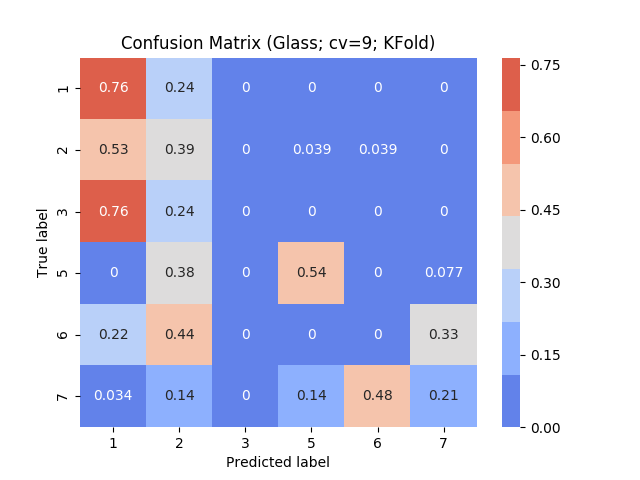
\includegraphics[width=\textwidth]{img/conf_matrices/cm_Glass_cv9_KFold.png}
    \caption{Macierz konfuzji dla najlepszej wartości F1 -- kroswalidacja zwykła.}
\end{figure}
        \pagebreak
Po zastosowaniu kroswalidacji stratyfikowanej wyniki dla zbioru danych \textbf{Glass},
poprawiły się niemal dwukrotnie. Miara F1 osiąga wartości rzędu 60\%. Dodatkowo jeszcze
bardziej uwidacznia się przewaga CAIM nad brakiem dyskretyzacji -- prawie 1,5 raza lepsze
wyniki. Dla metod \textit{equal-width} oraz \textit{equal-frequency} osiągane wyniki
pozostały niesatysfakcjonujące, co można tłumaczyć małą liczbą grup kroswalidacyjnych
(tylko dwie grupy).

\begin{figure}[H]
\center
    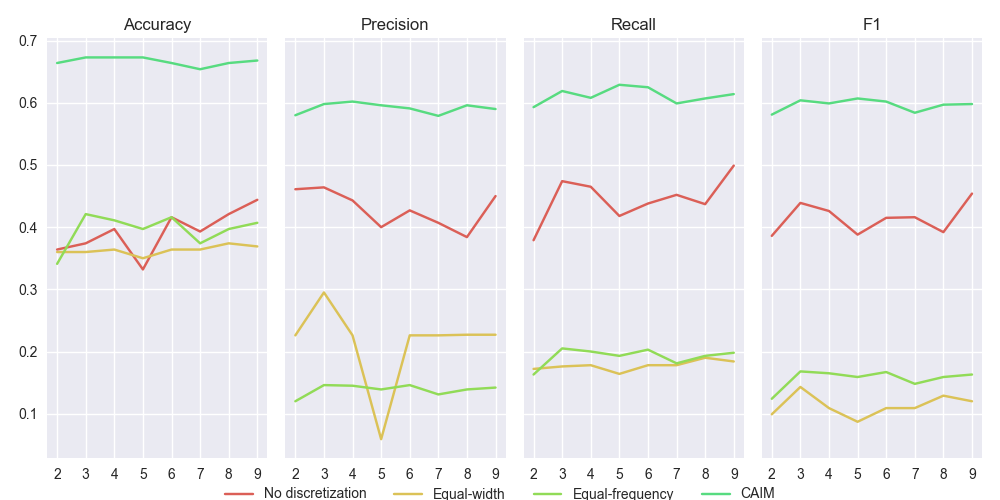
\includegraphics[width=\textwidth]{img/cv_scores_stratifiedkfold/scoring_stratifiedkfold_glass.png}
    \caption{Wykresy wartości metryk dla zbioru "Glass" -- kroswalidacja stratyfikowana.}
\end{figure}

Poprawę jakości uczenia klasyfikatora przy kroswalidacji stratyfikowanej, można zaobserwować również
na przykładzie macierzy konfuzji (wybranej dla parametru $K = 5$). Wartości wzdłuż przekątnej ("prawidłowe"
klasyfikacje) są wyraźnie wyższe i zatem lepsze.

\begin{figure}[H]
\center
    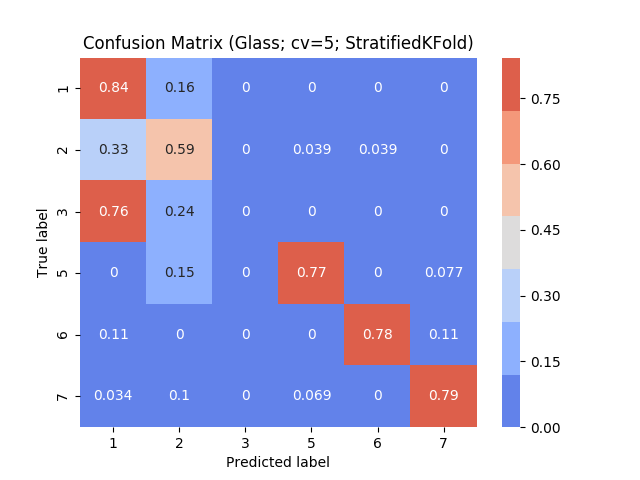
\includegraphics[width=0.6\textwidth]{img/conf_matrices/cm_Glass_cv5_StratifiedKFold.png}
    \caption{Macierz konfuzji dla najlepszej wartości F1 -- kroswalidacja stratyfikowana.}
\end{figure}


\begin{table}[H]
\center
    \caption{Wartości metryk dla zbioru "Glass" -- kroswalidacja stratyfikowana.}
    \begin{tabular}{|c|c|c|c|c|c|c|c|c|c|}
        \hline
        \multirow{2}{*}{\textbf{Metoda dyskr.}} & \multirow{2}{*}{\textbf{Metryka}} & \multicolumn{8}{|c|}{\textbf{CV}} \\ \cline{3-10}
                        &  & 2 & 3 & 4 & 5 & 6 & 7 & 8 & 9 \\ \hline
        \multirow{4}{*}{\textit{Brak}}  & Accuracy & 0.364 & 0.374 & 0.397 & 0.332 & 0.416 & 0.393 & 0.421 & 0.444 \\ \cline{2-10}
                                         & Precision & 0.461 & 0.464 & 0.443 & 0.4 & 0.427 & 0.407 & 0.384 & 0.45 \\ \cline{2-10}
                                         & Recall & 0.379 & 0.474 & 0.465 & 0.418 & 0.438 & 0.452 & 0.437 & 0.499 \\ \cline{2-10}
                                         & F1 & 0.386 & 0.439 & 0.426 & 0.388 & 0.415 & 0.416 & 0.392 & 0.454 \\ \hline \hline


        \multirow{4}{*}{\textit{Equal-width}}  & Accuracy & 0.36 & 0.36 & 0.364 & 0.35 & 0.364 & 0.364 & 0.374 & 0.369 \\ \cline{2-10}
                                             & Precision & 0.226 & 0.295 & 0.226 & 0.059 & 0.226 & 0.226 & 0.227 & 0.227 \\ \cline{2-10}
                                             & Recall & 0.172 & 0.176 & 0.178 & 0.164 & 0.178 & 0.178 & 0.19 & 0.184 \\ \cline{2-10}
                                             & F1 & 0.099 & 0.143 & 0.109 & 0.087 & 0.109 & 0.109 & 0.129 & 0.12 \\ \hline \hline


        \multirow{4}{*}{\textit{Equal-freq}}  & Accuracy & 0.341 & 0.421 & 0.411 & 0.397 & 0.416 & 0.374 & 0.397 & 0.407 \\ \cline{2-10}
                                             & Precision & 0.12 & 0.146 & 0.145 & 0.139 & 0.146 & 0.131 & 0.139 & 0.142 \\ \cline{2-10}
                                             & Recall & 0.163 & 0.205 & 0.2 & 0.193 & 0.203 & 0.181 & 0.193 & 0.198 \\ \cline{2-10}
                                             & F1 & 0.124 & 0.168 & 0.165 & 0.159 & 0.167 & 0.148 & 0.159 & 0.163 \\ \hline \hline


        \multirow{4}{*}{\textit{CAIM}}  & Accuracy & 0.664 & 0.673 & 0.673 & 0.673 & 0.664 & 0.654 & 0.664 & 0.668 \\ \cline{2-10}
                                     & Precision & 0.58 & 0.598 & 0.602 & 0.596 & 0.591 & 0.579 & 0.596 & 0.59 \\ \cline{2-10}
                                     & Recall & 0.593 & 0.619 & 0.608 & 0.629 & 0.625 & 0.599 & 0.607 & 0.614 \\ \cline{2-10}
                                     & F1 & 0.581 & 0.604 & 0.599 & 0.607 & 0.602 & 0.584 & 0.597 & 0.598 \\ \hline \hline

            \hline
    \end{tabular}
\end{table}


    \pagebreak
    \subsubsection{Zbiór danych -- "Wine"}
        \begin{figure}[H]
    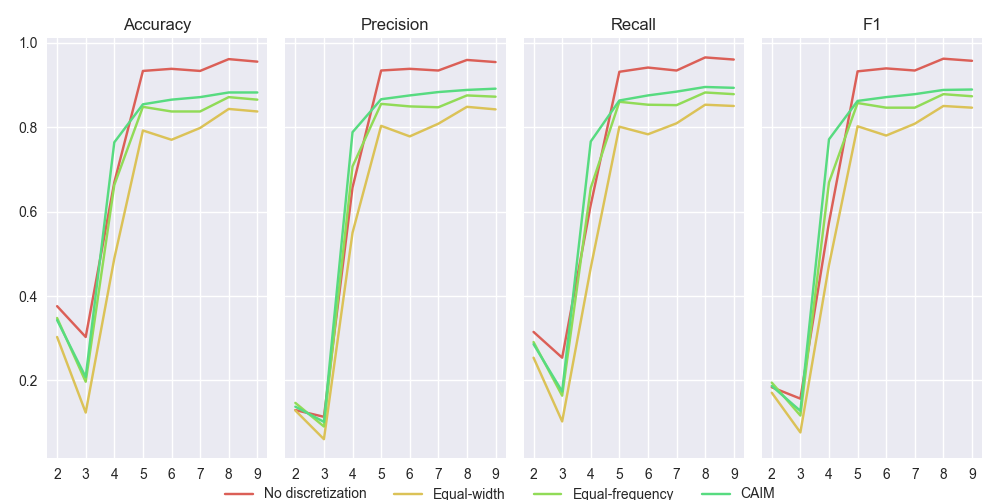
\includegraphics[width=\textwidth]{img/cv_scores_kfold/scoring_kfold_wine.png}
    \caption{Wykresy wartości metryk dla zbioru "Wine" -- krowalidacja zwykła.}
\end{figure}

        \begin{table}[H]
        \center
        \caption{Wartości metryk dla zbioru "Wine" -- krowalidacja zwykła.}
        \begin{tabular}{|c|c|c|c|c|c|c|c|c|c|}
            \hline
            \multirow{2}{*}{\textbf{Metoda dyskr.}} & \multirow{2}{*}{\textbf{Metryka}} & \multicolumn{8}{|c|}{\textbf{CV}} \\ \cline{3-10}
                            &  & 2 & 3 & 4 & 5 & 6 & 7 & 8 & 9 \\ \hline
            \multirow{4}{*}{\textit{Brak}}  & Accuracy & 0.376 & 0.303 & 0.669 & 0.933 & 0.938 & 0.933 & 0.961 & 0.955 \\ \cline{2-10}
                                             & Precision & 0.13 & 0.114 & 0.657 & 0.934 & 0.938 & 0.934 & 0.959 & 0.954 \\ \cline{2-10}
                                             & Recall & 0.315 & 0.254 & 0.616 & 0.931 & 0.941 & 0.934 & 0.965 & 0.96 \\ \cline{2-10}
                                             & F1 & 0.184 & 0.157 & 0.574 & 0.932 & 0.939 & 0.934 & 0.962 & 0.957 \\ \hline \hline


                                            \multirow{4}{*}{\textit{Equal-width}}  & Accuracy & 0.303 & 0.124 & 0.489 & 0.792 & 0.77 & 0.798 & 0.843 & 0.837 \\ \cline{2-10}
                                             & Precision & 0.129 & 0.061 & 0.55 & 0.803 & 0.778 & 0.808 & 0.848 & 0.842 \\ \cline{2-10}
                                             & Recall & 0.254 & 0.103 & 0.467 & 0.801 & 0.783 & 0.809 & 0.853 & 0.85 \\ \cline{2-10}
                                             & F1 & 0.171 & 0.077 & 0.473 & 0.802 & 0.78 & 0.808 & 0.85 & 0.846 \\ \hline \hline


                                            \multirow{4}{*}{\textit{Equal-freq}}  & Accuracy & 0.348 & 0.197 & 0.663 & 0.848 & 0.837 & 0.837 & 0.871 & 0.865 \\ \cline{2-10}
                                             & Precision & 0.147 & 0.091 & 0.707 & 0.855 & 0.849 & 0.847 & 0.875 & 0.872 \\ \cline{2-10}
                                             & Recall & 0.291 & 0.164 & 0.656 & 0.86 & 0.853 & 0.852 & 0.882 & 0.878 \\ \cline{2-10}
                                             & F1 & 0.195 & 0.117 & 0.669 & 0.857 & 0.846 & 0.846 & 0.878 & 0.873 \\ \hline \hline


                                            \multirow{4}{*}{\textit{CAIM}}  & Accuracy & 0.343 & 0.208 & 0.764 & 0.854 & 0.865 & 0.871 & 0.882 & 0.882 \\ \cline{2-10}
                                             & Precision & 0.138 & 0.102 & 0.788 & 0.866 & 0.875 & 0.883 & 0.888 & 0.891 \\ \cline{2-10}
                                             & Recall & 0.286 & 0.174 & 0.766 & 0.863 & 0.875 & 0.884 & 0.895 & 0.893 \\ \cline{2-10}
                                             & F1 & 0.187 & 0.128 & 0.771 & 0.862 & 0.871 & 0.878 & 0.888 & 0.889 \\ \hline \hline

            \hline
        \end{tabular}
    \end{table}

\begin{figure}[H]
    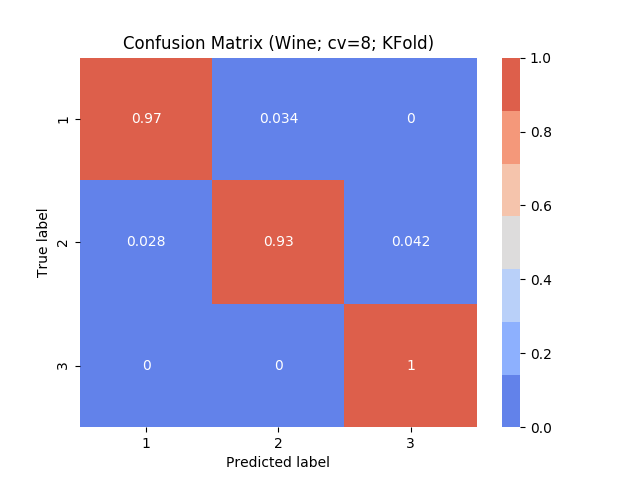
\includegraphics[width=\textwidth]{img/conf_matrices/cm_Wine_cv8_KFold.png}
    \caption{Macierz konfuzji dla najlepszej wartości F1 -- kroswalidacja zwykła.}
\end{figure}
        \subsection*{Kroswalidacja stratyfikowana}

\begin{figure}[H]
\center
    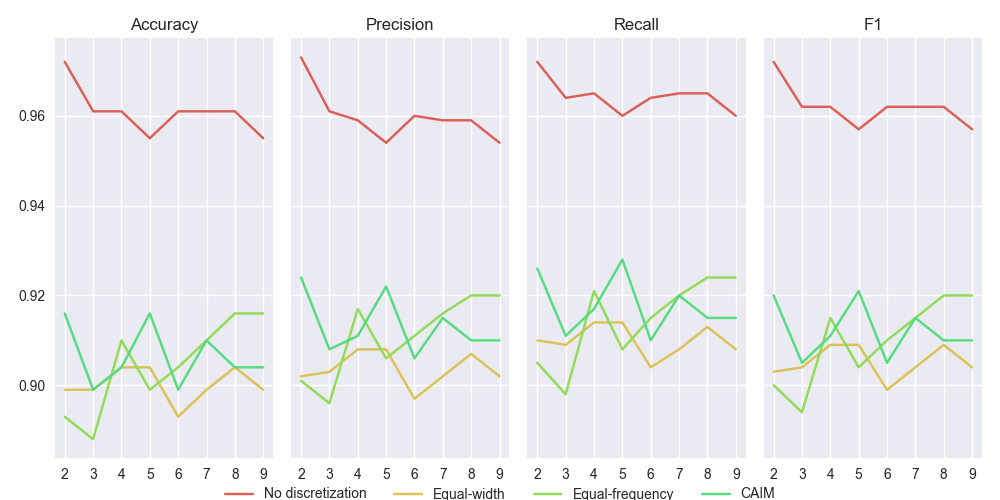
\includegraphics[width=0.9\textwidth]{img/cv_scores_stratifiedkfold/scoring_stratifiedkfold_wine.png}
    \caption{Wartości metryk dla klasyfikatora Bayesowskiego.}
\end{figure}

\begin{figure}[H]
    \center
    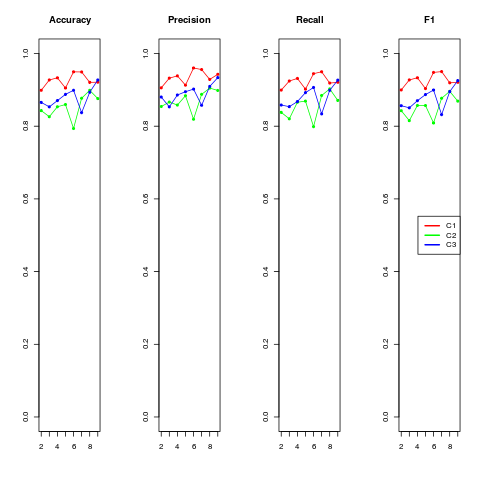
\includegraphics[width=0.8\textwidth]{img/cv_plots/cv_s_wine.png}
    \caption{Wartości metryk dla drzewa decyzyjnego C4.5.}
\end{figure}

\begin{table}[H]
  \center
  \begin{tabular}{|c|c|c|c|c|c|}
    \hline
    Klasyfikator & Accuracy & Precision & Recall & F1 & Komentarz \\ \hline
    Bayes        & 0.97     & 0.97      & 0.97   & 0.97 & Brak dyskretyzacji; K = 2 \\ \hline
    C4.5         & 0.95     & 0.96      & 0.95   & 0.95 & C1; K = 7 \\ \hline
  \end{tabular}

  \caption{Najlepsze wyniki dla klas. Bayesowskiego i drzewa C4.5 (względem F1).}
\end{table}

\begin{table}[H]
  \center
\begin{tabular}{|c|c|c|c|c|c|c|c|c|c|}  \hline
  \multicolumn{2}{|c|}{} & \multicolumn{8}{c|}{Liczba foldów} \\ \hline
Konfiguracja &    Metryka &     2 &     3 &     4 &     5 &     6 &     7 &     8 &     9 \\ \hline
          C1 &   Accuracy &  0.90 &  0.93 &  0.93 &  0.91 &  0.95 &  0.95 &  0.92 &  0.92 \\ \hline
          C1 &  Precision &  0.91 &  0.93 &  0.94 &  0.91 &  0.96 &  0.96 &  0.93 &  0.94 \\ \hline
          C1 &     Recall &  0.90 &  0.92 &  0.93 &  0.90 &  0.94 &  0.95 &  0.92 &  0.92 \\ \hline
          C1 &         F1 &  0.90 &  0.93 &  0.93 &  0.90 &  0.95 &  0.95 &  0.92 &  0.92 \\ \hline \hline
          C2 &   Accuracy &  0.84 &  0.83 &  0.85 &  0.86 &  0.79 &  0.88 &  0.90 &  0.88 \\ \hline
          C2 &  Precision &  0.85 &  0.87 &  0.86 &  0.88 &  0.82 &  0.89 &  0.90 &  0.90 \\ \hline
          C2 &     Recall &  0.84 &  0.82 &  0.87 &  0.87 &  0.80 &  0.88 &  0.90 &  0.87 \\ \hline
          C2 &         F1 &  0.84 &  0.82 &  0.86 &  0.86 &  0.81 &  0.88 &  0.90 &  0.87 \\ \hline \hline
          C3 &   Accuracy &  0.87 &  0.85 &  0.87 &  0.89 &  0.90 &  0.84 &  0.89 &  0.93 \\ \hline
          C3 &  Precision &  0.88 &  0.85 &  0.89 &  0.89 &  0.90 &  0.86 &  0.91 &  0.93 \\ \hline
          C3 &     Recall &  0.86 &  0.85 &  0.87 &  0.89 &  0.91 &  0.83 &  0.90 &  0.93 \\ \hline
          C3 &         F1 &  0.86 &  0.85 &  0.87 &  0.89 &  0.90 &  0.83 &  0.90 &  0.93 \\ \hline
\end{tabular}


  \caption{Dokładne wartości metryk dla drzewa decyzyjnego C4.5.}
\end{table}


